\documentclass[tikz,border=2pt]{standalone}
\usepackage{amsmath}
\usetikzlibrary{arrows.meta}
\begin{document}
% Sample path of L(t) on [0,10]: arrivals at 1,2,4,8, departures at 3,6,7, so the time in states
% 0, 1, 2 is Y(n,10) = 2, 5, 3 and the empirical fractions Y(n,10)/10 are 0.2, 0.5, 0.3.
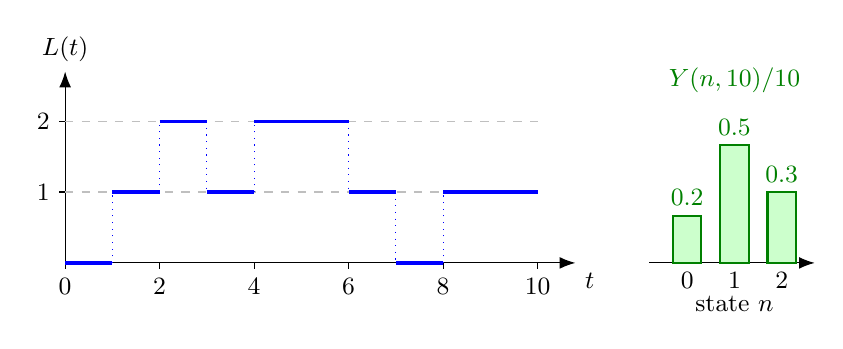
\begin{tikzpicture}[font=\small, >={Latex[length=2mm]}, x=0.6cm, y=0.9cm]
  % ---------- sample path ----------
  \draw[->] (0,0) -- (10.8,0) node[anchor=north west] {$t$};
  \draw[->] (0,0) -- (0,2.7) node[anchor=south] {$L(t)$};
  \foreach \x in {0,2,4,6,8,10} \draw (\x,0) -- (\x,-0.08) node[anchor=north] {$\x$};
  \foreach \y in {1,2} {
    \draw (0,\y) -- (-0.12,\y) node[anchor=east] {$\y$};
    \draw[gray!50, thin, dashed] (0,\y) -- (10,\y);
  }
  \draw[blue, very thick] (0,0) -- (1,0) (1,1) -- (2,1) (2,2) -- (3,2) (3,1) -- (4,1)
    (4,2) -- (6,2) (6,1) -- (7,1) (7,0) -- (8,0) (8,1) -- (10,1);
  \draw[blue, thin, dotted] (1,0) -- (1,1) (2,1) -- (2,2) (3,2) -- (3,1) (4,1) -- (4,2)
    (6,2) -- (6,1) (7,1) -- (7,0) (8,0) -- (8,1);
  % ---------- empirical fractions ----------
  \begin{scope}[xshift=7.6cm, y=3cm]
    \draw[->] (-0.3,0) -- (3.2,0);
    \foreach \n/\v in {0/0.2,1/0.5,2/0.3} {
      \fill[green!20] (\n+0.2,0) rectangle (\n+0.8,\v);
      \draw[green!50!black, thick] (\n+0.2,0) rectangle (\n+0.8,\v);
      \node[green!50!black, anchor=south] at (\n+0.5,\v) {$\v$};
      \node[anchor=north] at (\n+0.5,0) {$\n$};
    }
    \node[anchor=north] at (1.5,-0.1) {state $n$};
    \node[green!50!black, anchor=south] at (1.5,0.68) {$Y(n,10)/10$};
  \end{scope}
\end{tikzpicture}
\end{document}
